\documentclass{article}
\usepackage{graphicx}
\usepackage{booktabs}
\usepackage{multirow}
\usepackage{ctex}
\usepackage{amsmath}
\usepackage{geometry}
\geometry{a4paper, left=2.5cm, right=2.5cm, top=2.5cm, bottom=2.5cm}

\title{深度学习导论实验报告 \\ 作业1-2: 手写数字识别CNN模型分析}
\author{PB22000150-刘行}
\date{\today}

\begin{document}
\maketitle

	\section{实验原理}
		\subsection{卷积神经网络基本原理}
			卷积神经网络 (CNN) 通过局部连接和权值共享特性, 能有效提取图像空间特征. 本实验模型包含以下组件:

			\begin{itemize}
				\item \textbf{卷积层}: 使用 $3 \times 3$ 卷积核, padding 保持特征图尺寸
				\item \textbf{批归一化}: 加速训练并提升模型泛化能力
				\item \textbf{池化层}: 采用最大池化 (max) 或平均池化 (avg), 下采样率为 2
				\item \textbf{Dropout}: 在全连接层前以 0.5 概率随机失活神经元
				\item \textbf{激活函数}: ReLU 非线性激活
			\end{itemize}

			模型通过交叉熵损失函数和Adam优化器进行端到端训练.

	\section{模型分析}
		\subsection{AutoCNN详细结构}
			模型由特征提取器和分类器组成,以输入尺寸 $1\times28\times28$  为例:
			
			\textbf{特征提取器} (以\texttt{conv\_channels=[16,32]}为例):
			\begin{enumerate}
				\item \textbf{第一卷积模块}:
				\begin{itemize}
					\item Conv2d($1 \to 16$, kernel=$3 \times 3$, padding = 1): 输出尺寸 $16 \times 28 \times 28$
					\item BatchNorm2d(16): 引入 32 个可学习参数 (16个$\gamma$ + 16个$\beta$)
					\item ReLU 激活: $f\left(x\right) = \max\left(0, x\right)$
					\item MaxPool2d($2 \times 2$): 下采样至 $16 \times 14 \times 14$
				\end{itemize}
				
				\item \textbf{第二卷积模块}: 
				\begin{itemize}
					\item Conv2d($16 \to 32$, kernel=$3 \times 3$, padding=1):输出尺寸$32 \times 14 \times 14$
					\item BatchNorm2d(32): 引入 64 个参数
					\item ReLU 激活
					\item MaxPool2d($2 \times 2$):最终特征图尺寸$32 \times 7 \times 7$
				\end{itemize}
			\end{enumerate}
			
			\textbf{分类器}:
			\begin{itemize}
				\item Flatten 层: 将 $32 \times 7 \times 7$ 展平为 1568 维向量
				\item 全连接层 1: $1568 \to 128$, 参数量$1568 \times 128 + 128 = 200,832$
				\item ReLU 激活 + Dropout(0.5)
				\item 全连接层2: $128 \to 10$, 参数量$128 \times 10 + 10 = 1,290$
			\end{itemize}
		
		\subsection{参数量计算}
			总参数量由各层累加:
			\begin{equation*}
				\begin{aligned}
					\text{卷积层} & : (3^2\times1\times16) + (3^2\times16\times32) = 144 + 4,608 = 4,752 \\
					\text{BatchNorm} & : (16 + 32)\times2 = 96 \\
					\text{全连接层} & : 200,832 + 1,290 = 202,122 \\
					\hline
					\text{总计} & : 4,752 + 96 + 202,122 = 206,970
				\end{aligned}
			\end{equation*}
		
		\subsection{设计特性分析}
			\begin{itemize}
				\item \textbf{深度与感受野}: 2 层卷积 + 池化使感受野达到 $7 \times 7$, 可捕获数字整体结构
				\item \textbf{通道扩展策略}: 通道数 $16 \to 32$ 逐层加倍, 平衡计算量与特征表达能力
				\item \textbf{正则化配置}: BatchNorm 稳定训练过程, ropout 仅在分类器中使用以避免过度抑制浅层特征
			\end{itemize}

	\section{实验过程}
		\subsection{数据集与实验设置}
			使用 MNIST 数据集, 按以下比例划分:
			\begin{itemize}
				\item 训练集: 60000张 (原数据全部)
				\item 验证集: 10000张 (训练集 $\frac{1}{6}$)
				\item 测试集: 10000张 (原测试集全部)
			\end{itemize}

			\noindent 对比实验配置 (下页表 \ref{tab:config}):
			\begin{table}[htbp]
				\centering
				\caption{实验参数配置对比}
				\begin{tabular}{lcccc}
					\toprule
					配置项 & 基准配置 & 变体 1 & 变体 2 & 变体 3 \\
					\midrule
					池化方式 & max & avg & max & avg \\
					卷积通道 & [16,32] & [16,32] & [16,32,64] & [16,32,64] \\
					BatchNorm & 启用 & 启用 & 启用 & 启用 \\
					Dropout & 禁用 & 禁用 & 禁用 & 禁用 \\
					学习率 & 1e-4 & 1e-4 & 1e-4 & 1e-4 \\
					\bottomrule
				\end{tabular}
				\label{tab:config}
			\end{table}

		\subsection{训练策略调整}
			\begin{itemize}
				\item 初始设置 epochs=60, 发现验证准确率在 30 epoch 后趋于稳定 (图 \ref{fig:epoch60}, 在最后)
				\item 调整 epochs=30 以避免过拟合, 最终结果见图 \ref{fig:epoch30} (图在最后)
				\item 早停策略: 保存验证集最佳模型
			\end{itemize}

	\section{实验结果}
		\subsection{配置对比分析}
			\begin{table}[htbp]
				\centering
				\caption{不同配置下测试准确率对比}
				\begin{tabular}{lcc}
					\toprule
					配置描述 & 验证集最佳准确率 & 测试集准确率 \\
					\midrule
					max 池化 +2 层卷积 & 0.9903 & 0.9901 \\
					avg 池化 +2 层卷积 & 0.9915 & 0.9915 \\
					max 池化 +3 层卷积 & 0.9913 & 0.9916 \\
					avg 池化 +3 层卷积 & 0.9930 & 0.9936 \\
					\bottomrule
				\end{tabular}
			\end{table}

			关键发现:
				\begin{itemize}
					\item 深层网络 (3层卷积) 提升了性能, 验证准确率提高 $0.15\%$, 占错误率的 $15\%$, 效果有限
					\item avg 池化优于 max 池化, 测试准确率提高 $0.20\%$, 占错误率的 $24\%$
					\item 错误样本分析: 易混淆数字对为 $(9 \to 4)$, $(5 \to 3)$
				\end{itemize}

		\subsection{错误样本可视化}
			典型错误案例如图\ref{fig:errors}所示, 可见模糊书写和非常规字型是主要错误来源.

			\begin{figure}[htbp]
				\centering
				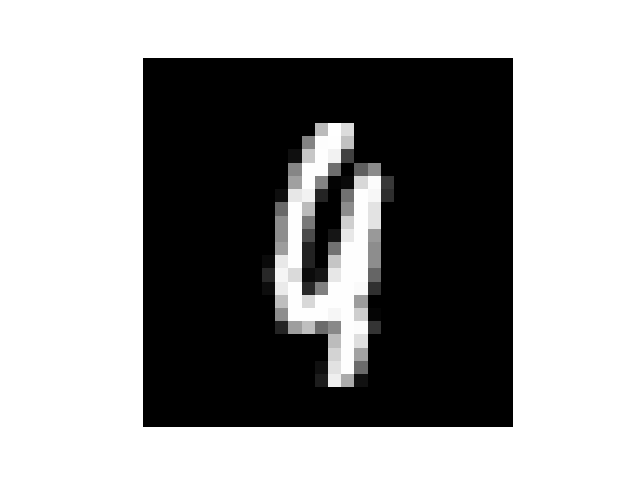
\includegraphics[width=0.19\textwidth]{figure/error_14_true9_predict4.png}
				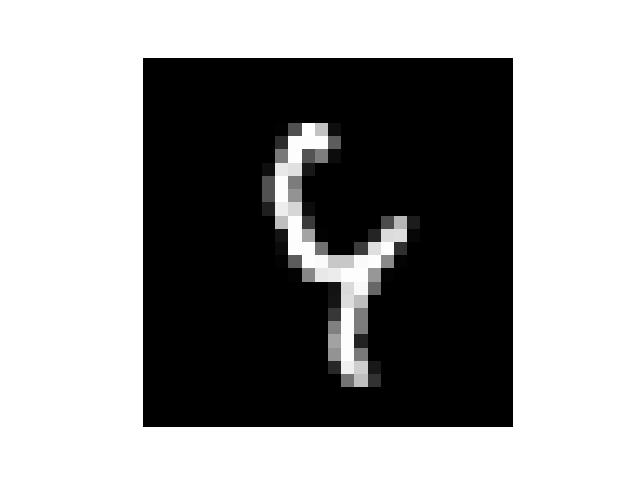
\includegraphics[width=0.19\textwidth]{figure/error_21_true9_predict4.png}
				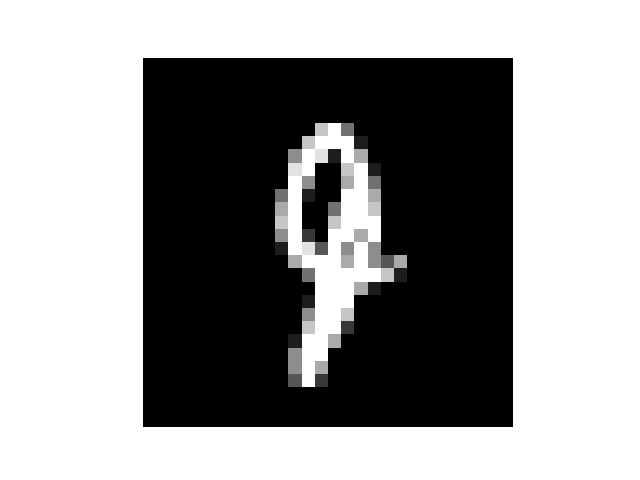
\includegraphics[width=0.19\textwidth]{figure/error_26_true9_predict4.png}
				
\includegraphics[width=0.19\textwidth]{figure/error_28_true2_predict0.png}
				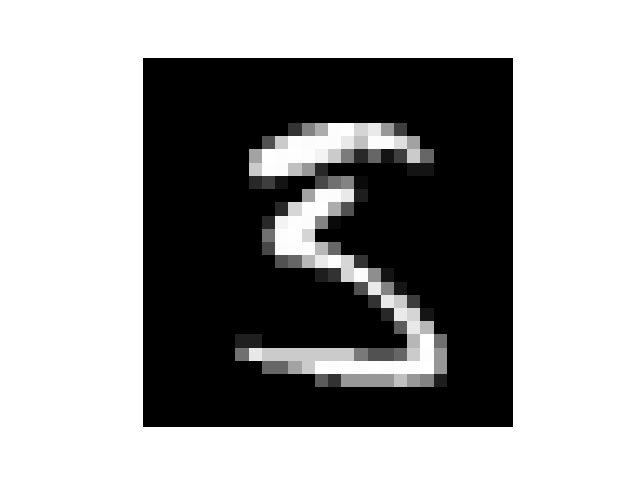
\includegraphics[width=0.19\textwidth]{figure/error_29_true5_predict3.png}
				\caption{典型错误分类样本 (真值→预测: 9→4*3, 2→0, 5→3)}
				\label{fig:errors}
			\end{figure}

	\section{结论}
		\begin{itemize}
			\item 适当降低模型深度 (2层卷积) 可平衡准确率与过拟合风险
			\item max池化在本任务中表现更优, 可能与数字图像的局部特征重要性相关
			\item 30epoch训练即可达到模型性能饱和, 延长训练易导致计算资源浪费
			\item 后续可尝试引入数据增强策略以提升小样本下的泛化能力
		\end{itemize}

	\section{图表}
		\begin{figure}[htbp]
			\centering
			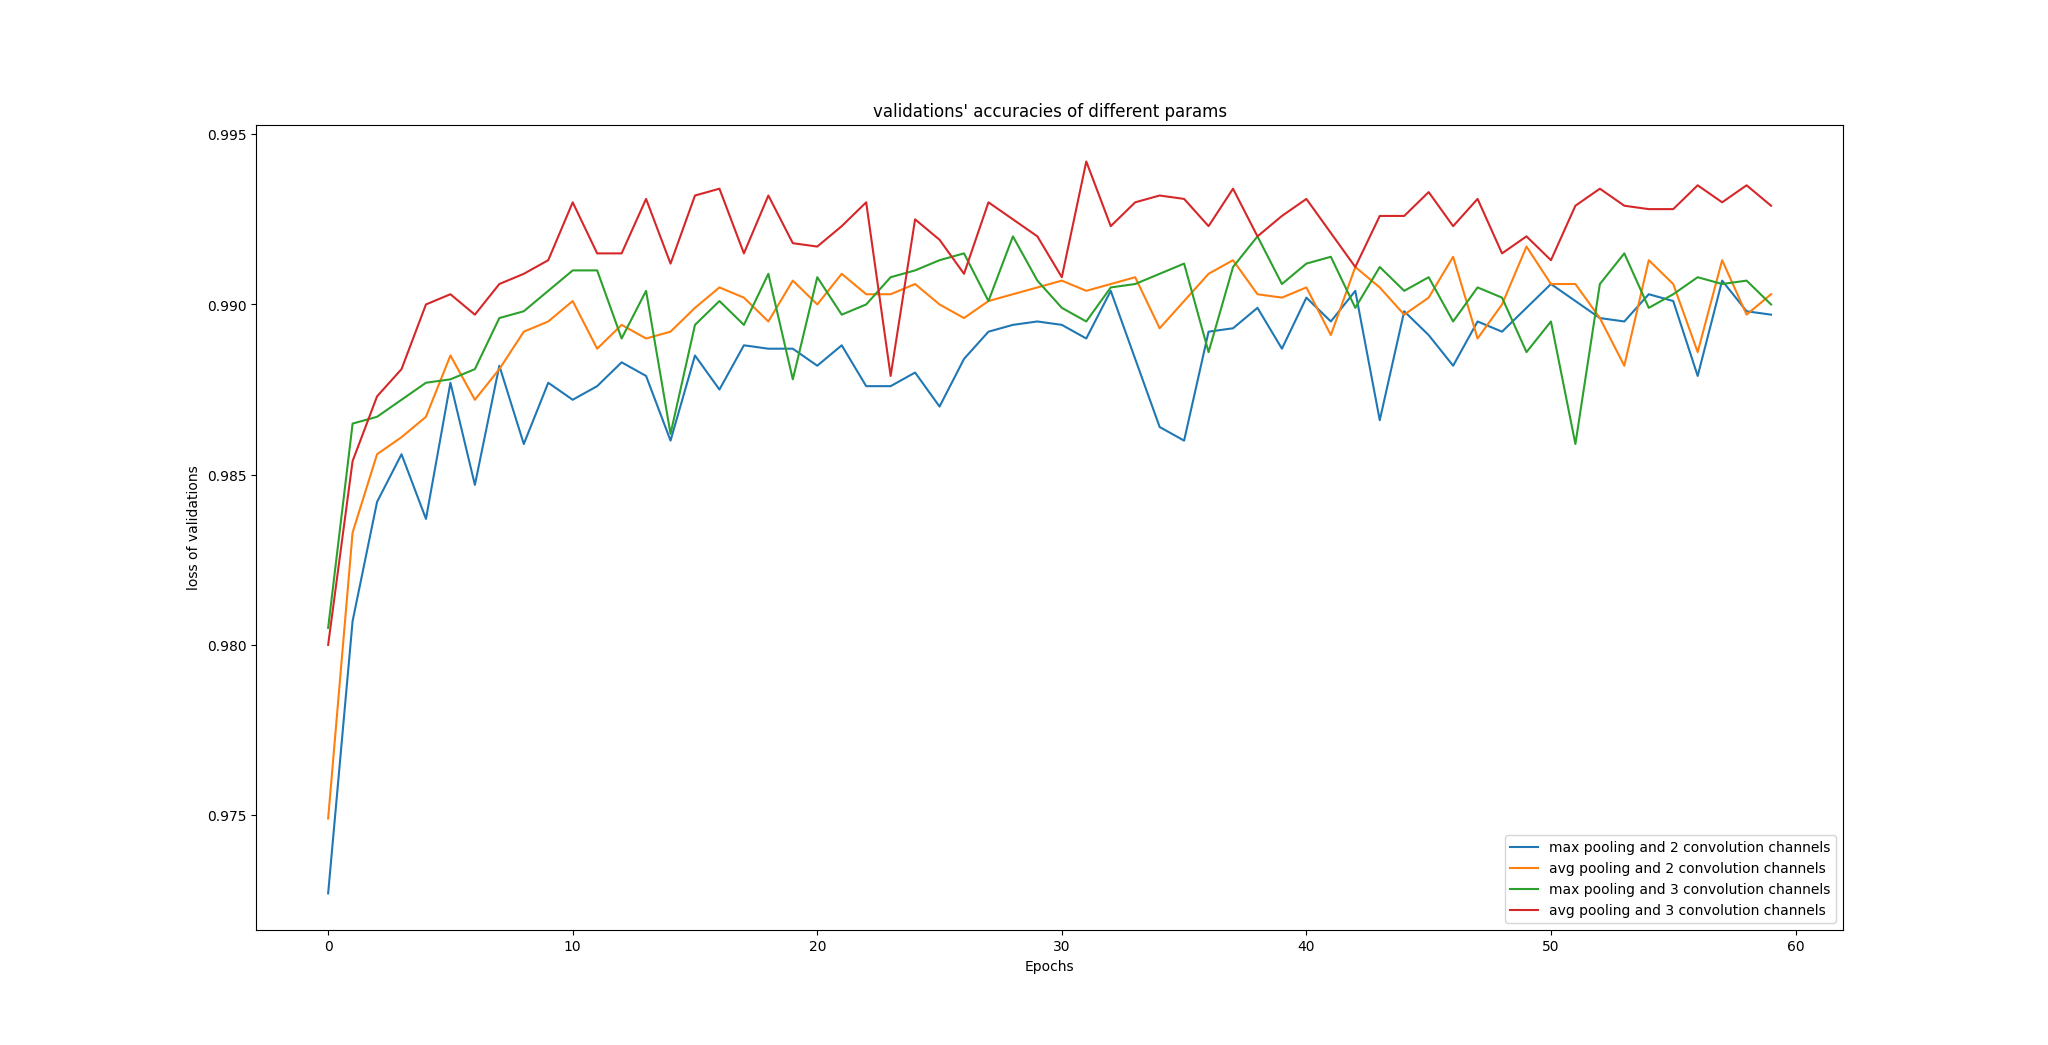
\includegraphics[width=0.8\textwidth]{figure/epochs_60_100_acc.png}
			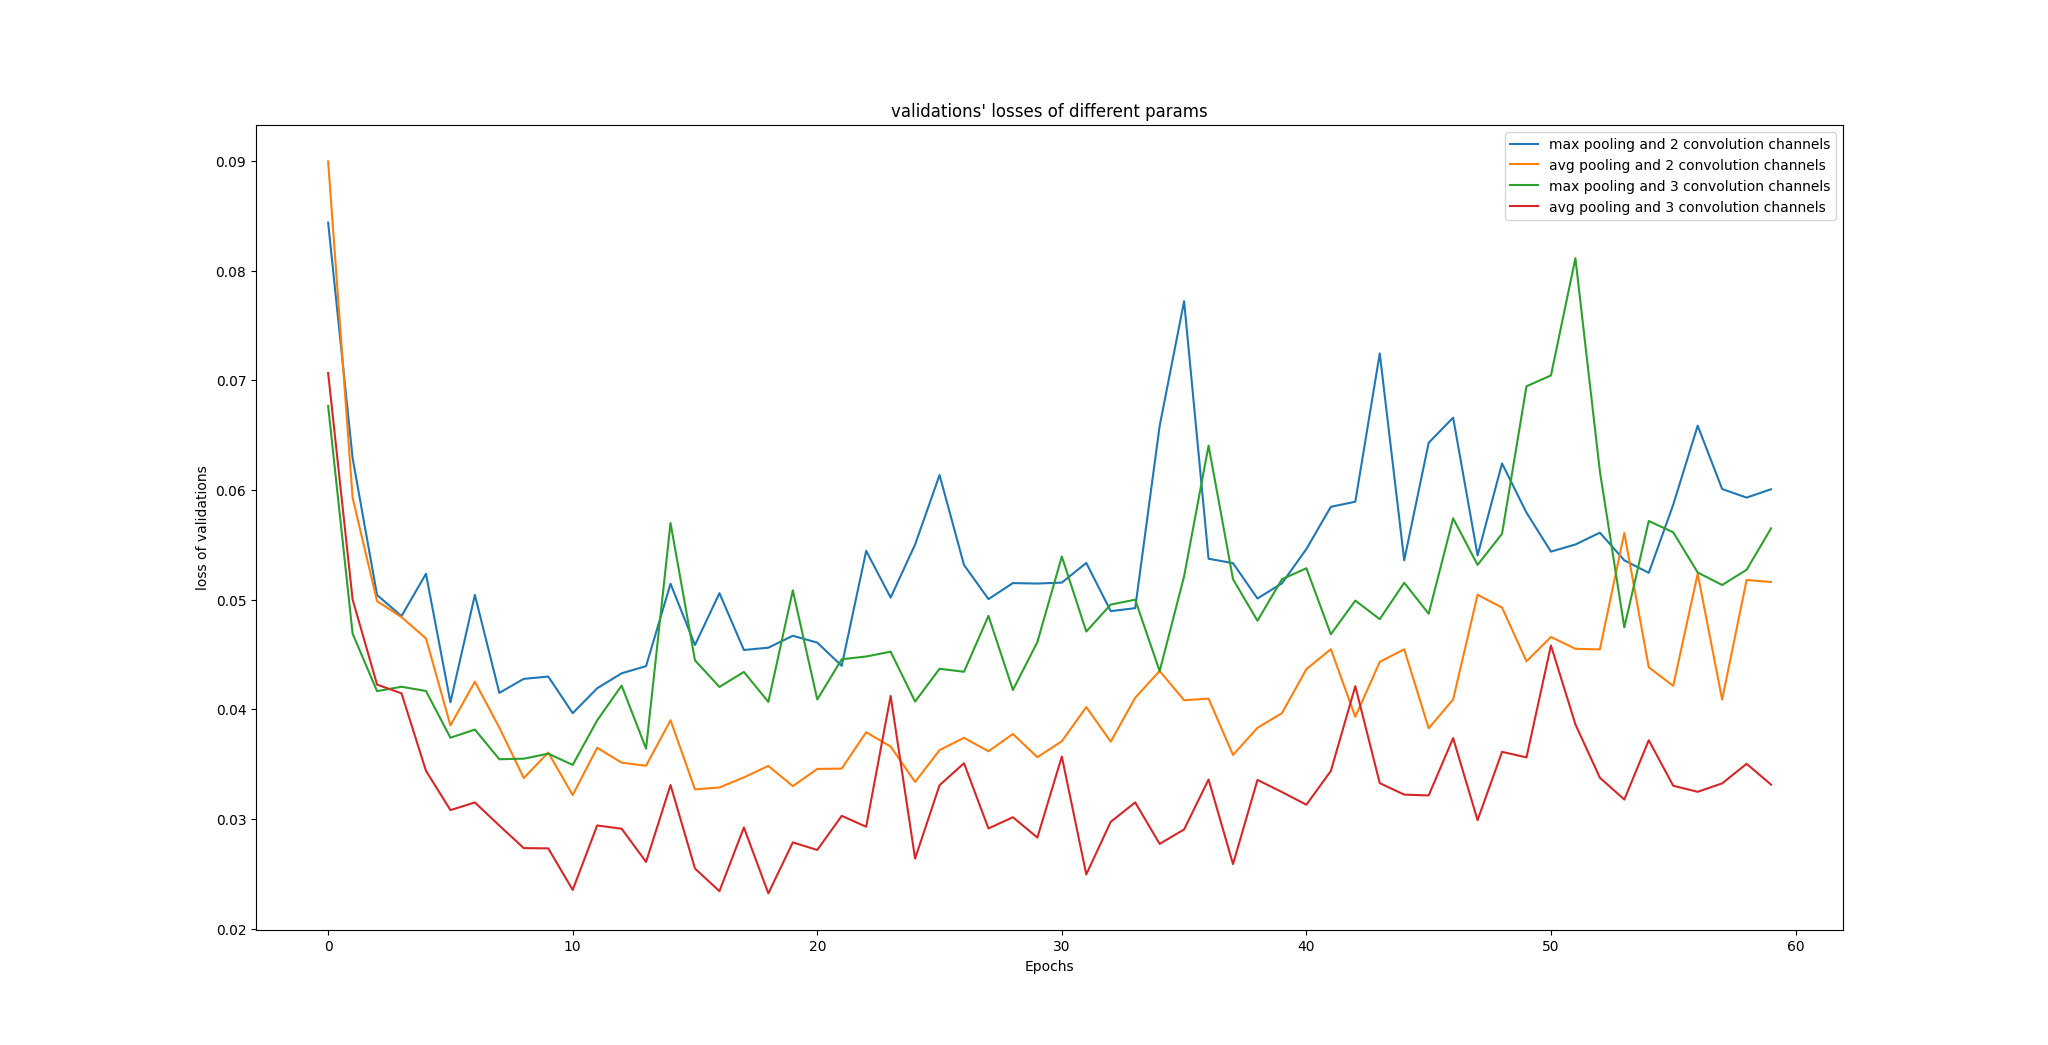
\includegraphics[width=0.8\textwidth]{figure/epochs_60_100_loss.png}\label{fig:epoch60}
			\caption{不同参数设置验证误差对比 (60epochs)}
		\end{figure}

		\begin{figure}[htbp]
			\centering
			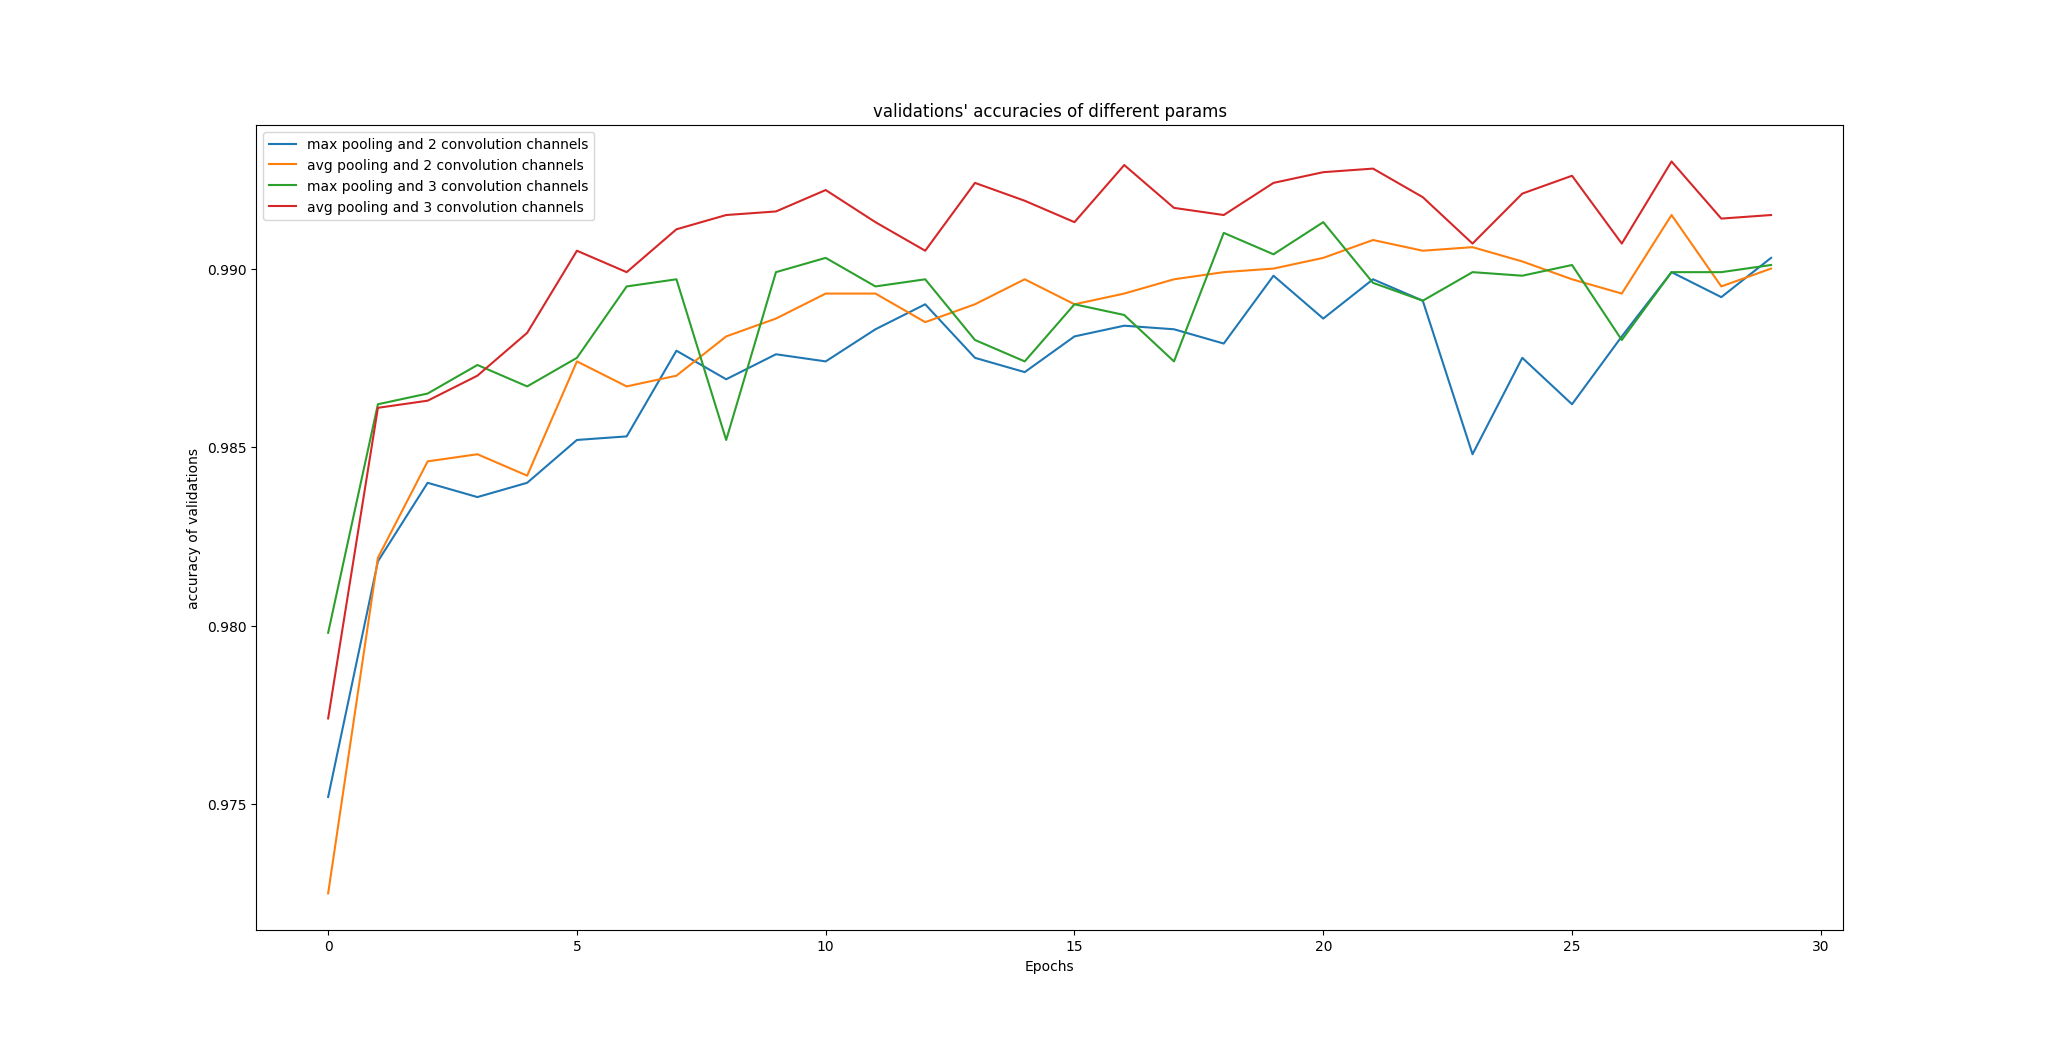
\includegraphics[width=0.8\textwidth]{figure/epochs_30_100_acc.png}
			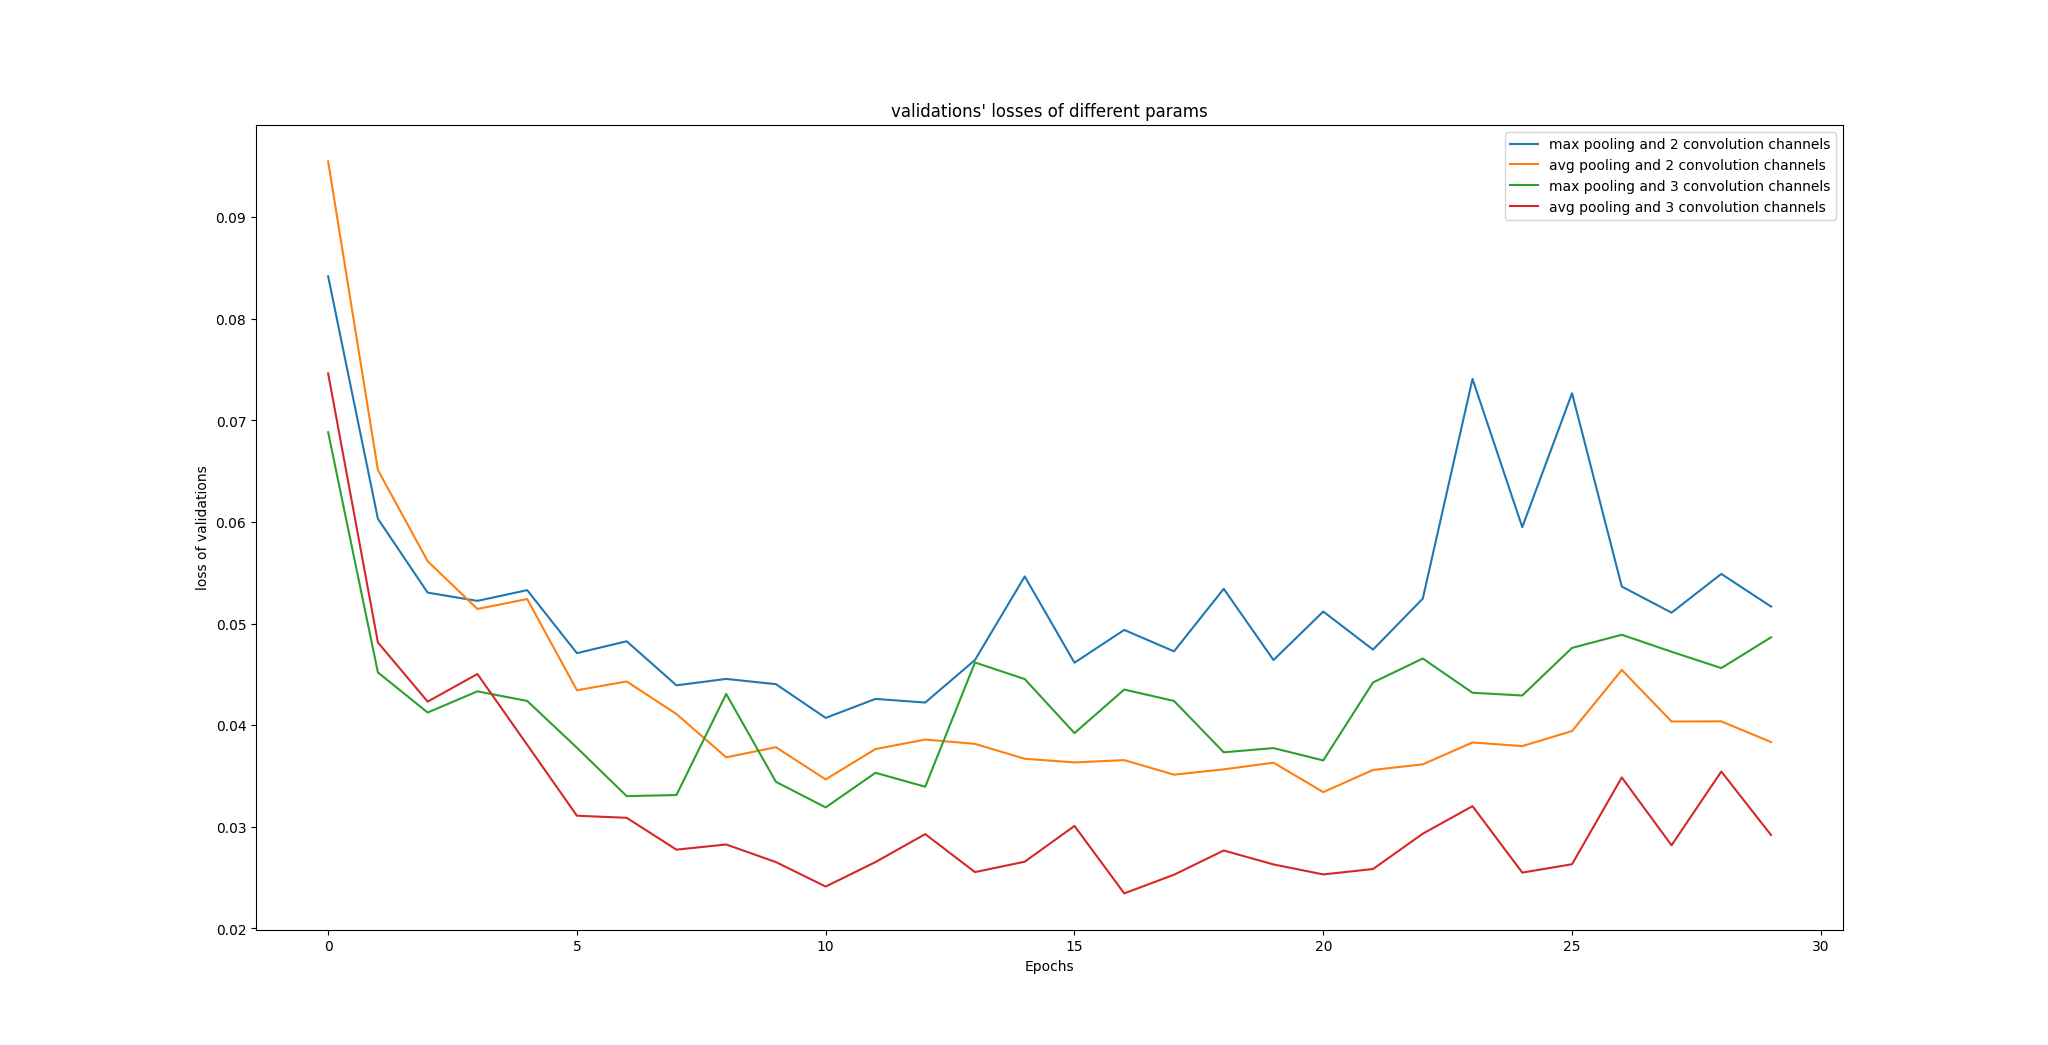
\includegraphics[width=0.8\textwidth]{figure/epochs_30_100_loss.png}\label{fig:epoch30}
			\caption{不同参数设置验证误差对比 (30epochs)}
		\end{figure}

\end{document}
